\section{Naming}\label{capitolo6}
I nomi giocano un ruolo importante in tutti i sistemi di computer. Sono utilizzati per identificare, condividere e localizzare le diverse risorse. Un elemento importante del naming riguarda il fatto che un nome può essere risolto nell'entità a cui si riferisce, consentendo così ad un processo di accedere alla risorsa identificata da quel nome.\\
La differenza tra il \emph{naming} nei sistemi distribuiti e nei sistemi non distribuiti è data dal modo in cui questi sistemi sono implementati. In un sistema distribuito molte volte anche il meccanismo di \emph{naming} è distribuito per migliorarne efficienza e scalabilità.\\
Esistono diversi meccanismi di naming quelli che analizzeremo saranno quelli di tipo \emph{human-friendly} come quelli dei file system o del World Wild Web. L'altro meccanismo di naming che analizzeremo è quello relativo al naming di dispositivi mobili dove i nomi human-friendly non sono adatti ma sono utilizzati meccanismi in cui i nomi sono identificatori indipendenti dalla posizione oppure quelli che utilizzano hash table distribuite.
Infine analizzeremo quella tipologia di naming che esprimono le entità tramite varie caratteristiche attraverso l'utilizzo di attributi.
\subsection{Nomi,identificatori ed indirizzi}
Definiamo innanzi tutto che cos'è un nome. Un nome in un sistema distribuito è una stringa di bit o di caratteri utilizzata per riferirsi ad una entità. Un'entità può essere qualsiasi cosa, come host, stampanti, dischi o file; ma anche qualcosa che conosciamo meglio come processi, utenti, pagine web ecc.\\
Con tali entità noi possiamo interagire ma per fare ciò è necessario accedervi tramite un \textbf{punto d'accesso} (\emph{access point}) che non è altro che un tipo particolare di entità il cui nome è anche chiamato \textbf{indirizzo.}\\
Un entità può avere più di un punto d'accesso e può cambiarlo nel corso del tempo. Un indirizzo perciò è un tipo speciale di nome che si riferisce al punto di accesso di un'entità. Visto che il punto di accesso è strettamente legato all'entità sarebbe opportuno utilizzare l'indirizzo come nome regolare per riferirsi all'entità. Questa tecnica non è però applicabile in quanto solitamente l'indirizzo non è di facile comprensione e nemmeno flessibile. Prendiamo ad esempio il caso in cui un sistema distribuito sia riorganizzato e che un servizio prima disponibile su di una macchina sia ora riassegnato ad un server differente supponiamo inoltre che sulla vecchia macchina venga messo in funzione un nuovo servizio; a questo punto se abbiamo utilizzato un indirizzo per riferirci all'entità nel momento in cui il punto di accesso cambia o viene riassegnato abbiamo un riferimento non valido.\\
Questo esempio illustra come per un entità un nome differente dal suo indirizzo sia più facile e più flessibile. Tale tipologia di nome è detta \textbf{indipendente dalla posizione}.\\
Oltre agli indirizzi ci sono altri tipi di nomi che meritano una piccola analisi e sono quelli utilizzati per identificare univocamente un'entità. Questi nomi sono detti \textbf{identificatori} e rispettano le seguenti proprietà:
\begin{itemize}
\item un identificatore si riferisce al massimo ad una entità.
\item Ogni entità è referenziata da al massimo un identificatore.
\item Un identificatore si riferisce sempre alla stessa entità (non è mai riusato)
\end{itemize}
Usando gli identificatori diventa più facile riferirsi a un'entità in maniera non ambigua.\\
Indirizzi ed identificatori sono due importanti categorie di nomi impiegati per due scopi molto diversi. In numerosi sistemi tali nomi sono sono rappresentati in una forma leggibile dalla macchina ovvero sotto forma di bit. Al contrario i nomi \emph{\textbf{human-friendly}} sono rappresentati sotto forma di stringhe di caratteri in modo da essere usate dalle persone.\\
Il problema principale del naming risulta a questo punto essere quello di risolvere nomi e identificatori in indirizzi. In linea di principio un sistema di \emph{naming} mantiene un \textbf{collegamento nome-indirizzo} che nella sua forma più semplice è solo una tabella di coppie (\emph{nomi, indirizzo}). Tuttavia in sistemi distribuiti su di un ampia area geografica o di grandi dimensioni una tabella centralizzata non può funzionare.
Ciò che accade è che un nome viene scomposto in più parti e che la risoluzione del nome avviene in maniera ricorsiva
\subsection{Flat naming}
In precedenza abbiamo visto come gli identificatori sono adatti per rappresentare univocamente le entità tramite stringhe di bit molto semplici i quali per comodità vengono chiamati nomi non strutturati o semplici (\emph{flat}). Tali nomi non contengono alcuna informazione su come localizzare il punto d'accesso all'entità.
\subsubsection{Soluzioni semplici}
Analizziamo come primo meccanismo due semplici approcci per localizzare le entità in una rete locale.
\paragraph{Broadcasting e multicasting}
Consideriamo una rete che offre funzionalità di \emph{broadcasting} efficienti. Localizzare un'entità in tale ambiente è relativamente semplice, basta inviare un messaggio contenente l'identificatore dell'entità ad ogni macchina per verificare che tali macchine abbiano la risorsa. Solo le macchine che possono offrire un punto d'accesso per quella risorsa risponderanno al messaggio inviando l'indirizzo di quel punto d'accesso.\\
Questo principio è usato nel \textbf{protocollo di risoluzione degli indirizzi} (ARP \emph{address resolution protocol}) per trovare l'indirizzo a livello del collegamento dati \emph{(data-link)} di una macchina dato solo l'indirizzo IP.\\
In sostanza una macchina trasmette sulla rete locale un pacchetto richiedendo chi sia il proprietario di un determinato indirizzo IP. Quando un messaggio raggiunge una macchina controlla se ha l'indirizzo IP e in caso affermativo risponde al messaggio.\\
Tale meccanismo tuttavia diventa inefficiente man mano che la rete cresce, in quanto viene sprecata banda dalla grande quantità di messaggi inoltrati, inoltre molti host possono essere interrotti da richieste alle quali non possono dare una risposta. Una soluzione possibile è quella di passare al \emph{multicasting} nel quale solo un ristretto numero di host riceve la richiesta. Il \emph{multicasting} può essere usato per localizzare una risorsa nelle reti punto-a-punto, ad esempio, Internet supporta il \emph{multicasting} a livello di rete consentendo a diversi host di unirsi ad uno specifico gruppo di \emph{multicast}. Tali gruppi sono identificati da un \textbf{indirizzo multicast}. Quando un host invia un messaggio ad un indirizzo di multicast il livello di rete fornisce un meccanismo \emph{best-effort} per consegnare questo messaggio a tutti i membri del gruppo.\\
Un modo per utilizzare un indirizzo multicast potrebbe essere il caso di un azienda nel quale un PC,che chiameremo $A$, può essere connesso alla rete. Quando A viene connesso gli viene assegnato un indirizzo IP ed entra a far parte di un gruppo multicast. Nel caso un altro PC volesse contattare A dovrebbe prima di tutto localizzarlo e per fare ciò potrebbe inviare un messaggio "dov'è A?" a tutto il gruppo multicast, se A è connesso risponde con il suo indirizzo attuale.\\
Un altro modo per utilizzare un indirizzo di multicast è quello di associarlo ad un'entità replicata ed utilizzare il multicast per localizzare la replica più vicina.
\paragraph{Puntatori forwarding}
Un altro approccio molto diffuso per localizzare un'entità mobile è quella di utilizzare dei puntatori \emph{forwarding}. Il principio è abbastanza semplice, quando un'entità si sposta da A ad una nuova posizione B si lascia dietro un puntatore alla sua nuova posizione. Il vantaggio principale è la semplicità di realizzazione. Non appena viene trovata un'entità tramite \emph{naming service} tradizionale, un client può cercare l'indirizzo attuale seguendo la catena dei puntatori.\\
Esistono però anche una serie di inconvenienti; primo fra tutti se non vengono prese le opportune contromisure la catena di puntatori per un'entità molto mobile può diventare estremamente lunga e la sua localizzazione diventare molto dispendiosa. Inoltre ogni nodo intermedio della catena deve mantenere la sua parte di puntatori finché è necessario. Infine, il sistema è molto vulnerabile alla perdita di comunicazione, se viene perso uno dei puntatori la risorsa non è più raggiungibile. \uppercase{è} quindi fondamentale mantenere le catene di puntatori corte e i puntatori robusti.\\
Per capire il loro funzionamento prendiamo il caso dei puntatori \emph{forwarding} applicati agli oggetti remoti ai quali si accede tramite chiamate a procedure remote. Seguendo l'approccio delle \textbf{catene SSP} ogni puntatore è implementato come coppia (\emph{client stub, server stub}) come mostrato in \figurename\,\ref{img:forwarding}. Un server stub contiene un riferimento all'oggetto locale o un un riferimento ad un client stub remoto.\\
\begin{figure}
\centering
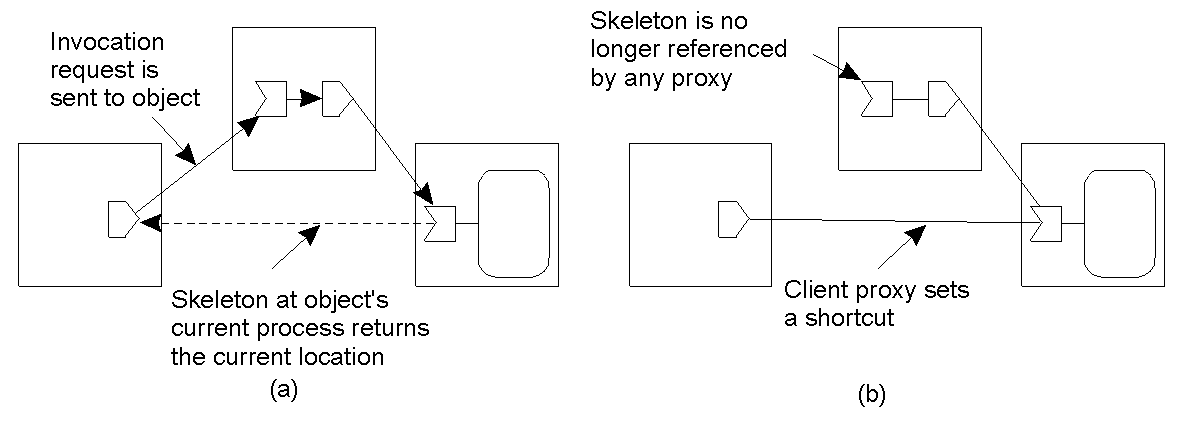
\includegraphics[scale=0.5]{img/forwarding.png}
\caption{Esempio di utilizzo di puntatori forwarding}\label{img:forwarding}
\end{figure}
Quando un oggetto si sposta dallo spazzio degli indirizzi di $A$ a quello di $B$ lascia su $A$ al suo posto un client stub che punta ad un server stub installato su $B$. Il punto focale è che la migrazione è completamente trasparente al client che contatta solo il client stub, gli è nascosto, invece, come e a quale posizione questo client inoltra le chiamate.\\
Per mantenere corta la catena una chiamata ad oggetto comporta l'identificazione del client che ha effettuato la chiamata tramite il suo indirizzo a livello di trasporto unito ad un numero generato localmente per identificare lo stub. Quando la chiamata arriva all'oggetto esso invia la risposta direttamente al client senza risalire la catena di puntatori, inoltre, insieme alla risposta viene inviata la posizione attuale dell'oggetto.\\
Si deve stabile un compromesso tra l'inviare una risposta direttamente al client stub oppure lungo la catena dei puntatori, nel primo caso la comunicazione è più veloce nel secondo invece è possibile aggiornare tutti i vari stub con la posizione aggiornata dell'oggetto.\\
Quando più nessun client fa riferimento ad un server stub, allora, quest'ultimo può essere rimosso. Tale operazione è strettamente collegata alla \emph{garbage collection} distribuita.
\subsubsection{Approcci home-based}
L'utilizzo del \emph{broadcasting} o di puntatori \emph{forwarding} comporta problemi di scalabilità. Un approccio diffuso per supportare entità mobili su reti di larga scala consiste nell'utilizzo della \textbf{home location} che tiene traccia della posizione attuale di un'entità. La home location di solito è il luogo dove è stata creata l'entità.\\
Il caso più comune nel quale si utilizzano gli approcci \emph{home-based} è quello dei Mobile IP dove ogni host ha un indirizzo IP fisso. Tutte le comunicazioni verso questo indirizzo viene inizialmente diretta verso \textbf{home agent} dell'host mobile. L'home agent è posizionato nella rete locale corrispondente all'indirizzo IP dell'host. Quando l'host mobile si sposta in un altra rete richiede un indirizzo temporaneo; questo \textbf{care-of-address} viene registrato dall'\emph{home agent}. Quando l'home agent riceve un pacchetto per l'host mobile cerca la posizione attuale dell'host, se l'host è nella rete locale allora il pacchetto semplicemente viene inoltrato, altrimenti, viene incanalato verso la posizione attuale dell'host e contemporaneamente il mittente del pacchetto viene informato sull'attuale posizione dell'host. Questo meccanismo è mostrato in \figurename\,\ref{img:homebase}.\\
\begin{figure}
\centering
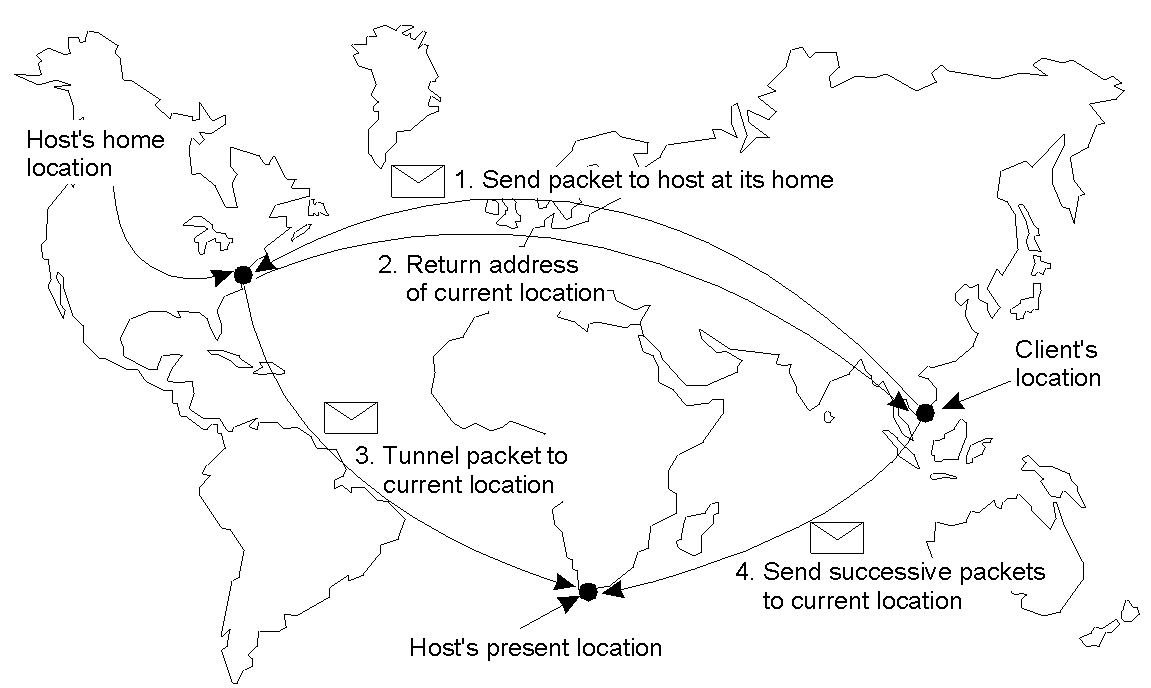
\includegraphics[scale=0.5]{img/homebase.png}
\caption{Il principio mobile IP}\label{img:homebase}
\end{figure}
Un inconveniente di questo meccanismo è che un host può essere molto lontano dalla sua home, il risultato è un aumento dei tempi di latenza. Inoltre, bisogna assicurare che la home location esista sempre altrimenti risulta impossibile contattare la risorsa.
\subsubsection{Hash table distribuite}
I recenti sviluppi hanno portato a possibili risoluzioni di un identficatore nell'indirizzo  di un elemento associato tramite l'utilizzo di \emph{hash table} distribuite. Nella concezione di base i meccanismi basati su SHT non tengono conto della vicinanza della rete, questo può causare problemi di prestazioni.
\paragraph{Meccanismo generale} 
Esistono diversi sistemi basati su DHT, il sistema \emph{Chord} è rappresentativo di molti di loro anche se esistono importanti differenze riguardo la complessità di gestione e i protocolli di ricerca.\\
Come abbiamo visto nel Capitolo \ref{capitolo2} Chord utilizza uno spazio degli identificatori a $m$ bit per assegnare degli identificatori casuali ai nodi e alle chiavi di una specifica entità. Il numero $m$ di bit è solitamente 128 o 160 a seconda della funzione di \emph{hash} utilizzata. Un'entità con chiave $k$ cade sotto la giurisdizione del nodo con il più piccolo identificatore $id \geq k$; questo nodo è chiamato il \emph{successore} di $k$ e indicato come $succ(k)$.\\
La questione principale in un sistema basato su DHT è quello di risolvere una chiave $k$ nell'indirizzo di $succ(k)$. Un approccio semplice ma che purtroppo non scala bene è di lasciare che ogni nodo $p$ tenga traccia del suo successore $succ(p+1)$ e del suo predecessore $pred(p)$. In questo caso quando un nodo $p$ riceve una richiesta la inoltra semplicemente ad uno dei suoi vicini a meno che la chiave che sta cercando non rispetti $pred(p) < k \leq p$, in questo caso il nodo $p$ deve restituire il suo indirizzo.\\
Diversamente da questo approccio lineare, ogni nodo Chord mantiene una \textbf{finger table} di al massimo $m$ elementi. Se $FT_p$ è la \emph{finger table} del nodo $p$ allora 
$$FT_p[i] = succ(p+2^{i-1})$$
Ovvero l'\emph{i-esimo} elemento punta al primo nodo successivo a $p$ di almeno $2^{i-1}$ posizioni. Questi riferimenti sono collegamenti a nodi realmente esistenti, dove la distanza del collegamento (\emph{short-cutted distance}) dal nodo $p$ cresce esponenzialmente man mano che aumenta l'indice della finger table.\\
Per individuare una chiave $k$ il nodo $p$ inoltra la richiesta al nodo $q$ con indice $j$ nella \emph{finger table} di $p$ dove
$$q = FT_p[j]\leq k < FT_p[j+1]$$
Per mostrare il funzionamento si rimanda alla \figurename\,\ref{img:chordexe} dove si mostrano i passaggi per la ricerca di una chiave $k = 7$ inoltrata al nodo 1.
Si può dimostrare che una ricerca richiede in genere $O(log(N))$ passi, dove $N$ sono il numero di nodi del sistema.\\
\begin{figure}
\centering
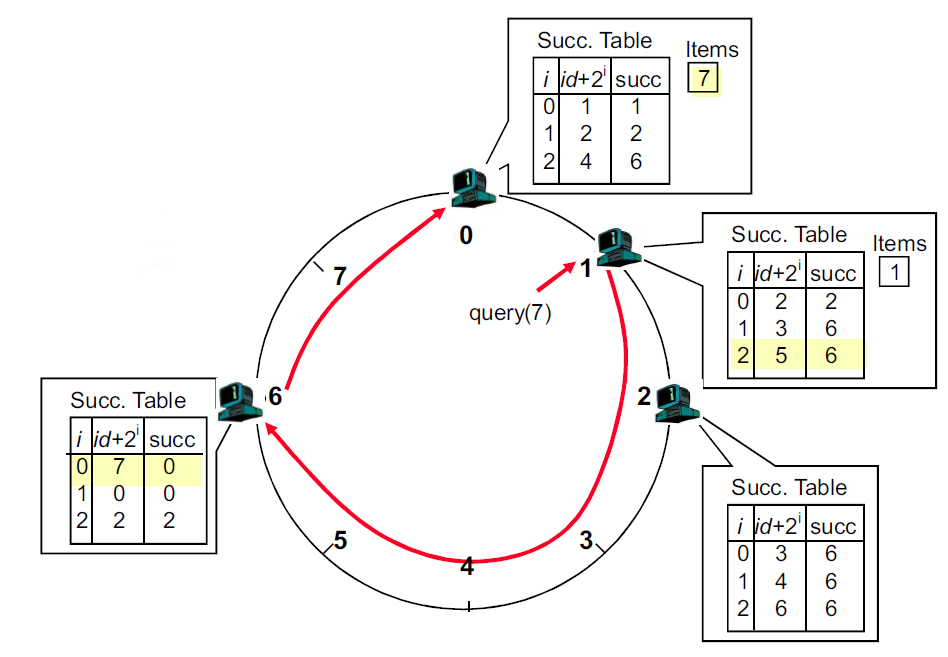
\includegraphics[scale=0.5]{img/chordexe.png}
\caption{Esempio di esecuzione di due ricerche}\label{img:chordexe}
\end{figure}
In un sistema distribuito ci si può aspettare che l'insieme dei nodi cambi continuamente, non solo i nodi entrano ed escono volontariamente ma possono anche subire dei guasti per poi tornare a funzionare successivamente.
Entrare in un sistema basato su DHT come \emph{Chord} è relativamente semplice. Supponiamo che un nodo $p$ voglia unirsi al sistema, esso contatta un nodo a caso del sistema e richiede la ricerca di $succ(p+1)$. Una volta identificato $p$ può unirsi all'anello. La complessità sta nel mantenere le \emph{finger table} aggiornate. La cosa più importante è che per ogni nodo $q$, $FT_q[1]$ (il successore) sia corretto. Per ottenere questo risultato ogni nodo $q$ esegue periodicamente una semplice procedura che contatta il $succ(q+1)$ e gli richiede di restituire $pred(succ(q+1))$. Se $q=pred(succ(q+1))$ allora $q$ è sicuro che le sue informazioni sono consistenti. Altrimenti nel sistema è entrato un nodo $p$ con $q<p\leq succ(q+1)$ per cui $q$ aggiornerà $FT_q[1]$ a $p$. A questo punto controllerà anche se $p$ ha memorizzato $q$ come suo predecessore. Se non fosse così allora è necessario un ulteriore aggiornamento di $FT_q[1]$.\\
Per aggiornare la finger table il nodo $q$ non deve far altro che contattare il successore di $k = q+2^{i-1}$ per ogni elemento $i$ della sua \emph{finger table}.
\paragraph{Sfruttare la vicinanza della rete}
Uno dei problemi principali del sistema Chord è che le richieste possono essere instradate in modo bizzarro, per minimizzare simili casi la progettazione di un sistema basato su DHT deve tener conto della rete sottostante.\\
Una prima soluzione potrebbe essere l'\textbf{assegnamento degli identificatori dei nodi basato sulla topologia}, in altre parole l'idea è quella di assegnare gli identificatori in modo tale che nodi vicini abbiano anche identificatori vicini. Questo meccanismo porta con sè però molte problematiche tra cui il \emph{mapping} di un anello logico su internet, che è un operazione non banale. Inoltre nel caso in cui una sottorete non diventi più raggiungibile si possono avere dei buchi consistenti negli identificatori che altrimenti avrebbero una distribuzione casuale.\\
Con l'\textbf{instradamento per vicinanza} (\emph{proximity routing}) i nodi mantengono una liste di alternative a cui inoltrare una richiesta. Per esempio preso un indice della finger table non si tiene conto solo del successore ma anche di $n$ successori nell'intervallo $[p+2^{i-1},p+2^i-1]$, ciò porta il sistema a poter scegliere a chi instradare una richiesta.\\
Infine nella \textbf{proximity neighbor selection} l'idea è quella di ottimizzare le tabelle di \emph{routing} in modo tale che il nodo più vicino sia selezionato come \emph{neighbor}. Non vi è molta differenza tra il \emph{proximity routing} e il \emph{proximity neighbor selection} in quanto nel proximity routing si scelgono $r$ alternative mentre nel proximity neighbor si scelgono gli $r$ vicini migliori.
\subsubsection{Approcci gerarchici}
L'approccio principale che presenteremo in questo paragrafo è basato sul servizio di localizzazione di \emph{Globe}. Si tratta di un servizio di localizzazione generico rappresentativo di molti sistemi di localizzazione gerarchici.\\
In uno schema gerarchico una rete è suddivisa in un insieme di \textbf{domini}. Esiste un solo dominio \emph{top-level} che comprende l'intera rete. Ogni dominio può essere suddiviso in molti sottodomini più piccoli, il dominio di livello più basso (\emph{lowest-level}) viene chiamato \textbf{dominio foglia} e corrisponde di solito ad una rete locale (LAN).\\
Ogni dominio $D$ ha un nodo directory associato $dir(D)$ che tiene traccia delle entità nel dominio. Questo meccanismo porta ad un albero di nodi directory con il nodo directory del dominio \emph{top-level} chiamato anche \textbf{nodo radice} il quale conosce tutte le entità. Tale organizzazione è mostrata in \figurename\,\ref{img:gerarchica}\\
\begin{figure}
\centering
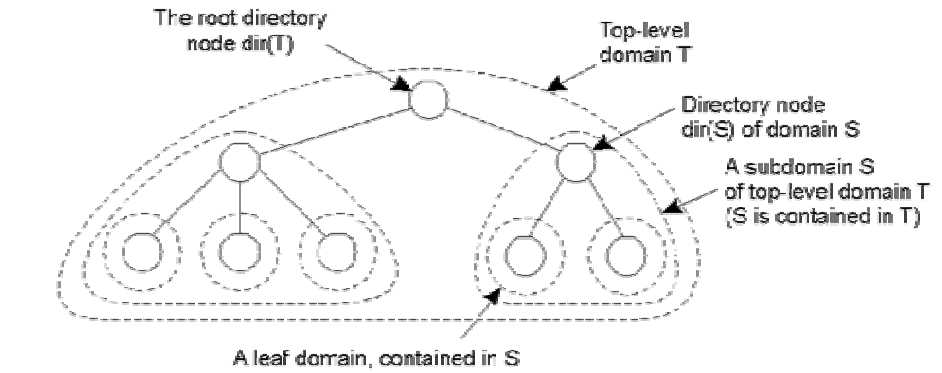
\includegraphics[scale=0.4]{img/gerarchico.png}
\caption{Esempio di organizzazione gerarchica}\label{img:gerarchica}
\end{figure}
Ogni entità attualmente posizionata in un dominio $D$ è rappresentata da un \textbf{location record} nel nodo directory $dir(D)$. Un \emph{location record} dell'entità $E$ nel nodo directory $N$ del dominio foglia $D$ contiene l'indirizzo attuale dell'entità in quel dominio. Mentre a livello superiore il \emph{location record} di $E$ conterrà un puntatore ad $N$.\\
Un'entità può avere molteplici indirizzi, ad esempio nel caso sia replicata. In tal caso il nodo directory del dominio più piccolo che contiene le due entità avrà due puntatori ai due sotto-domini per quell'entità coem mostrato in \figurename\,\ref{img:sottodomini}
\begin{figure}
\centering
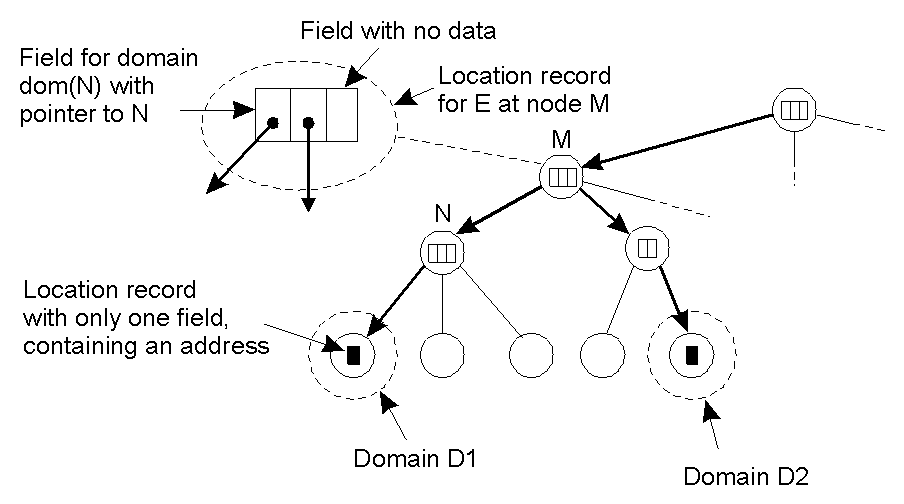
\includegraphics[scale=0.5]{img/sottodominio.png}
\caption{Esempio di memorizzazione delle informazioni nel caso di entità replicata}\label{img:sottodomini}
\end{figure}
Per quanto riguarda la ricerca in un sistema gerarchico avviene anch'essa in modo gerarchico ma con un approccio \emph{bottom-up}; se nel nodo directory non è presente un \emph{location record} per quell'entità allora il nodo inoltra la richiesta al padre, se anche il padre non ha un \emph{location record} per l'entità la richiesta risale l'albero fino a quando non trova un location record valido oppure non raggiunge la radice. Non appena una richiesta raggiunge un nodo directory $M$ contenente un \emph{location record} per l'entità $E$ sappiamo che $E$ si trova da qualche parte nel dominio $dom(M)$. A questo punto la richiesta viene inoltrata al nodo directory del sottodominio contente $E$ e così via procedendo fino a raggiungere una foglia, questo indirizzo può finalmente essere restituito al client che ha inoltrato la richiesta. Questo procedimento è illustrato in \figurename\,\ref{img:ricerca}
\begin{figure}
\centering
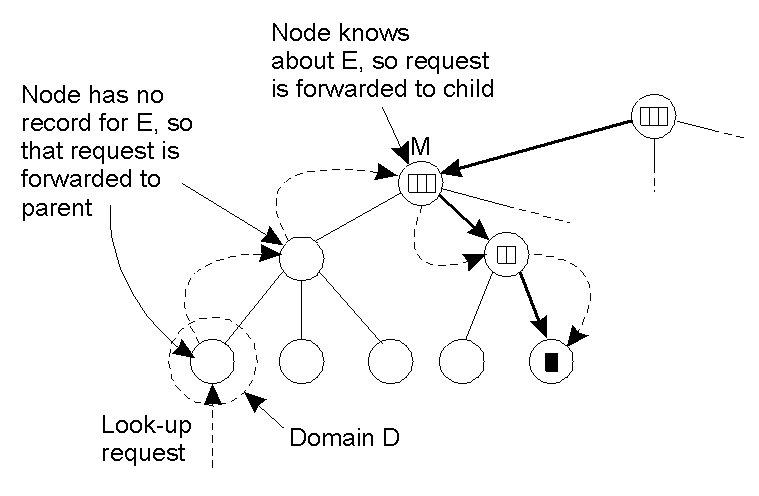
\includegraphics[scale=0.5]{img/ricerca.png}
\caption{Esempio di ricerca in un sistema gerarchico}\label{img:ricerca}
\end{figure}
Le operazioni di aggiornamento sfruttano lo stesso principio, l'inserimento avviene in un nodo foglia e il riferimento ad $E$ è propagato verso l'alto fino a quando in un nodo directory non si incontra già un riferimento ad $E$, a questo punto il nodo che ha già il \emph{location record} per e memorizza il nodo figlio dal quale è giunta la richiesta di inserimento, per installare la catena dei puntatori si possono applicare sia meccanismi \emph{top-down} (una volta raggiunto un nodo con un location record per $E$ si ridiscende l'albero impostando i diversi puntatori) oppure, un approccio \emph{bottom-up} (a mano a mano che la ricerca del location record di $E$ sale si instaurano i puntatori ad $E$). Nel secondo caso una risorsa diventa disponibile per un determinato dominio non appena la richiesta risale per il nodo directory di quel dominio.
\subsection{Naming strutturato}
I nomi semplici sono adatti per le macchine ma in generale non sono opportuni per gli uomini. Come alternativa i sistemi di \emph{naming} supportano i nomi strutturati composti da diversi nomi semplici e leggibili dall'uomo. Un esempio sono i nomi dei file, i nomi degli host di Internet e altri ancora.
\subsubsection{Name space}
I nomi sono solitamente organizzati nel cosiddetti \textbf{spazi dei nomi} o \emph{name space}. Uno spazio dei nomi può essere rappresentato come un grafo orientato nel quale esistono due tipi di nodi, i \textbf{nodi foglia} che rappresentano le diverse entità e può contenere soltanto informazioni come indirizzi, come nel caso di host oppure contenere direttamente tutto lo stato dell'entità come nel caso dei file system.\\
Esistono poi i \textbf{nodi directory} i quali hanno diversi archi in uscita ciascuno dei quali etichettato con un nome. Tuttavia questa è l'unica differenza in quanto in un grafo dei nomi ogni nodo è considerato come un'entità. Un nodo directory contiene una tabella in cui un arco in uscita è rappresentato da una coppia (\emph{etichetta dell'arco, identificatore del nodo}), tale tabella è chiamata \textbf{directory table}.\\
Un nodo che ha solo archi in uscita e nessun arco in entrata viene detto \textbf{nodo radice}. Ogni percorso in un grafo dei nomi può essere chiamato tramite una sequenza di etichette corrispondenti agli archi del percorso ad esempio
$$N:<label_1, label_2, \dots, label_n>$$
Tale percorso è detto \textbf{path name}. Se il primo nodo in un \emph{path name} è la radice del grafo è detto \textbf{path name assoluto} altrimenti è detto \textbf{path name relativo}.\\
Un \textbf{nome globale} è un nome che denota la stessa entità a prescindere da dove sia usato il nome all'interno del sistema. Diversamente un \textbf{nome locale} è un nome la cui interpretazione dipende da dove il nome viene usato. 
\subsubsection{Risoluzioni dei nomi}
Gli spazi dei nomi sono un meccanisomo adatto a memorizzare e recuperare informazioni sulle entità per mezzo dei nomi. Dato un path name dovrebbe essere possibile ricercare qualunque informazione memorizzata nel nodo cui il path name si riferisce. Il processo di ricerca in base a un nome è chiamato \textbf{risoluzione del nome} o \emph{name resolution}.\\
Per spiegare come funziona consideriamo il \emph{path name} precedente
$$N:<label_1, label_2, \dots, label_n>$$
La risoluzione di questo nodo comincia dal nodo $N$ del grafo dei nomi, viene poi ricercato il nodo con nome $label_1$ nella \emph{directory table}; ci si sposta poi in tale nodo e nella sua \emph{directory table} si ricerca il riferimento al nodo con nome $label_2$ e così via. Supponendo che tale path sia un percorso valido allora la risoluzione terminerà nell'ultimo nodo indicato da $label_n$ con la resttuzione del contenuto di quel nodo.
\paragraph{Meccanismo di chiusura}
La risoluzione di un nome può avvenire soltanto se sappiamo come e da dove iniziare, nel nostro esempio il nodo iniziale era specificato e sapevamo di aver accesso alla sua \emph{directory table}. Sapere come e da dove iniziare viene chiamato \textbf{meccanismo di chiusura}.\\
Un meccanismo di chiusura ha a che fare con la selezione del nodo iniziale in uno spazio dei nomi da cui deve iniziare la risoluzione. A volte però tali meccanismi sono di difficile comprensione in quanto molte volte impliciti e diversi gli uni dagli altri.\\
Per esempio nel file system di UNIX la risoluzione punta sul fatto che l'\emph{inode} della \emph{root directory} è il primo \emph{inode} nel disco logico.
\paragraph{Linking e mounting}
Strettamente correlato alla risoluzione dei nomi è l'uso di \textbf{alias}. Un alias è un altro nome per la stessa entità. Ad esempio una variabile d'ambiente come \texttt{\$HOME} è un esempio di alias. Ci sono fondamentalmente due modi per implementare un alias, il primo metodo è di consentire che molteplici path name assoluti si riferiscano allo stesso nodo  come mostrato in \figurename\,\ref{img:hardlink}. Questo approccio nei file system UNIX è chiamato \textbf{hard link}. 
\begin{figure}[htb]
\centering
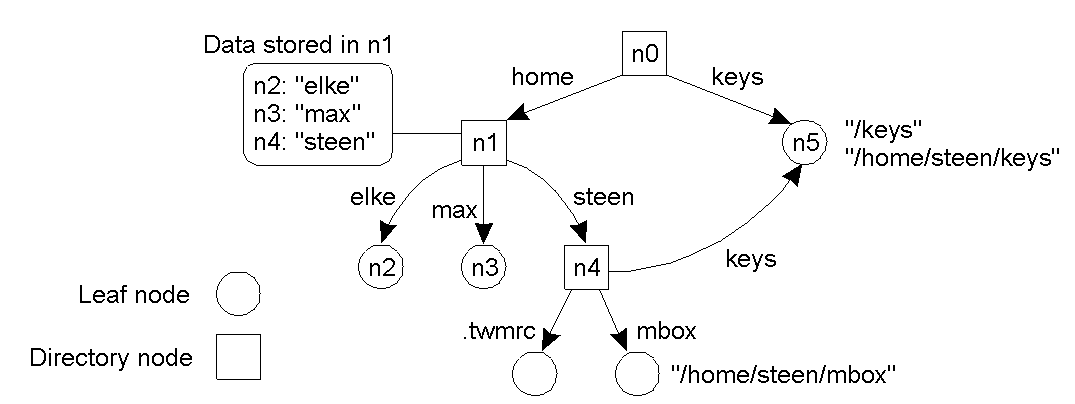
\includegraphics[scale=0.5]{img/hardlink.png}
\caption{Esempio di hard link}\label{img:hardlink}
\end{figure}
Il secondo metodo è quello di rappresentare un'entità tramite un nodo foglia il quale al posto di memorizzare l'indirizzo o lo stato dell'entità memorizza un path name assoluto come mostrato in \figurename\,\ref{img:symboliclink}. Questa volta, sempre riferendoci ai file system UNIX parliamo di \textbf{link simbolici}.
\begin{figure}[htb]
\centering
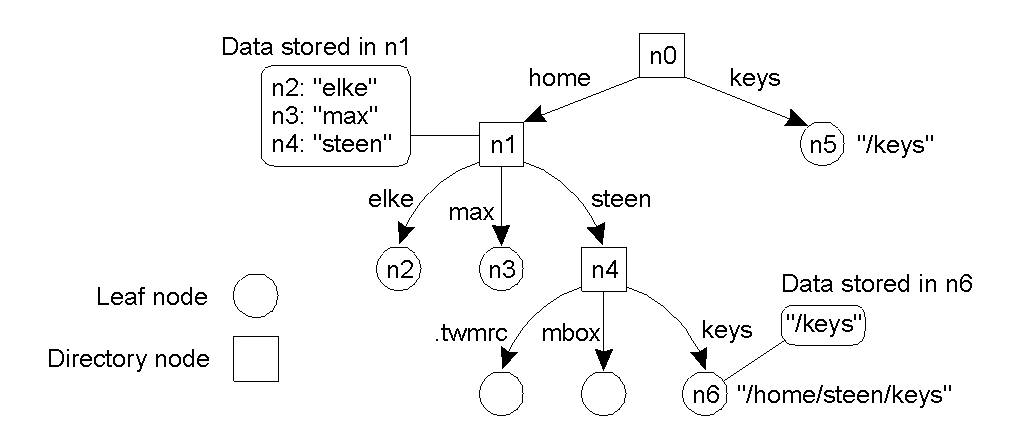
\includegraphics[scale=0.5]{img/symboliclink.png}
\caption{Esempio di hard link}\label{img:symboliclink}
\end{figure}
\subsubsection{Implementazione di uno spazio dei nomi}
Lo spazio dei nomi come abbiamo visto è il cuore di un \emph{naming service}. Un naming service è implementato da un name server. Se un sistema distribuito è limitato ad una rete locale è possibile implementare un name service mediante un unico name server centralizzato. Se invece il sistema ha molte entità ed è distribuito su larga scala allora è necessario distribuire il name server su più macchine.
\paragraph{Distribuzione dello spazio dei nomi}
Gli spazi dei nomi per sistemi distribuiti su larga scala sono solitamente organizzati gerarchicamente. Il \textbf{livello globale} è costituito dai nomi di più alto livello cioè il nodo radice ed i nodi directory logicamente più vicini ad essa. i nodi del livello globale sono spesso caratterizzati per la loro stabilità nel senso che le directory table cambiano raramente. Tali nodi possono rappresentare le aziende o i gruppi di aziende i cui nomi sono memorizzati nello spazio dei nomi.\\
Il \textbf{livello amministrativo} è costituito dai nodi directory gestiti da una sola azienda, questi nodi rappresentano gruppi di entità che appartengono alla stessa azienda o unità amministrativa, come un nodo per ogni per ogni dipartimento dell'azienda oppure uno utilizzato solo per gli utenti.\\
Il \textbf{livello gestionale} è il livello più basso ed è costituito da nodi che cambiano regolarmente. A questo gruppo appartengono gli host di una rete interna. Diversamente dagli altri livelli questi host sono gestiti non solo dagli amministratori ma anche dagli utenti finali.\\
La \figurename\,\ref{img:dnslevel} mostra una possibile suddivisione dello spazio dei nomi del DNS. Lo spazio dei nomi è diviso in parti non sovrapponibili chiamate \textbf{zone}. Una zona è uno spazio dei nomi che è implementato da un nameserver separato.
\begin{figure}
\centering
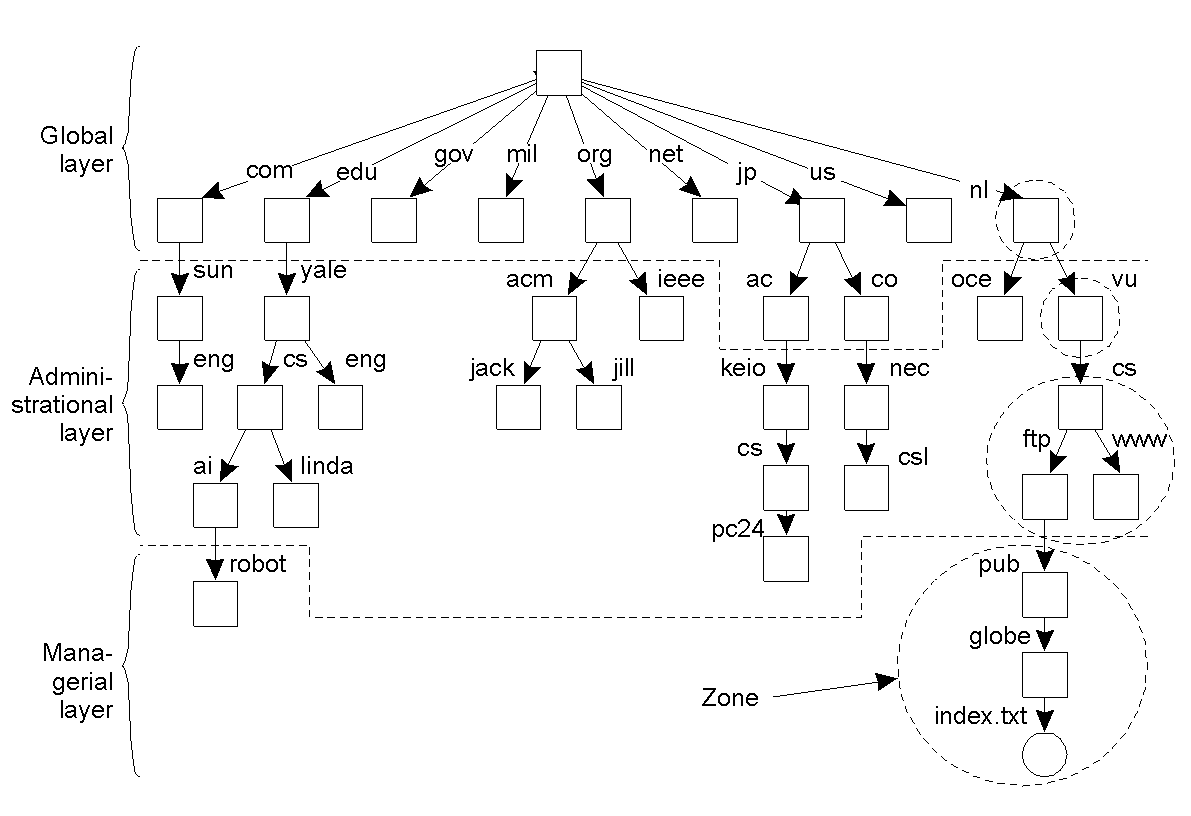
\includegraphics[scale=0.5]{img/dnslevel.png}
\caption{Esempio di suddivisione dei tre livelli nello spazio dei nomi del DNS}\label{img:dnslevel}
\end{figure}
Relativamente a disponibilità e prestazioni i name server dei diversi livelli devono rispettare diversi requisiti. I name server del livello globale devono essere altamente disponibili, in quanto se un name server si guasta un'ampia parte dello spazio dei nomi diventa irraggiungibile. Per quanto riguarda le prestazioni invece sono un po meno critiche in quanto cambiando raramente i risultati di ricerca possono essere memorizzati localmente dai client tramite meccanismi di cache. Il \emph{throughtput} però deve essere elevato in quanto le richieste provengono da una grande quantità di utenti. I requisiti di disponibilità e di prestazzioni per i server di livello globale possono essere soddisfatti replicando i server in combinazione con i meccanismi di cache.\\
La disponibilità dei name server a livello amministrativo è importante per i client all'interno della stessa azienda, infatti se si guasta le risorse all'interno dell'azienda diventano irraggiungibili. In merito alle prestazioni sono molto simili a quelle del livello globale in quanto anche qui i nodi non cambiano spesso, tuttavia, le tempistiche per i risultati delle ricerche devono essere nell'ordine di qualche millisecondo, anche gli aggiornamenti devono essere tempestivi, infatti, è inaccettabile che per l'attivazione di un account si debba aspettare qualche ora.\\
I requisiti prestazionali dei name server a livello gestionale sono molto più stringenti, la disponibilità non è importante ma le prestazioni sono una caratteristica molto importante in quanto gli utenti si aspettano che le operazioni avvengano immediatamente. Inoltre a causa dei continui aggiornamenti i meccanismi di cache lato client non sono efficaci e bisogna perciò interrogare sempre il nameserver.
\paragraph{Implementazione dello spazio dei nomi}
La distribuzione di uno spazio dei nomi su più \emph{name server} influenza l'implementazione della risoluzione dei nomi. Per spiegare la loro implemnetazione partiamo perciò dal caso più semplice in cui i name server non siano replicati ne che abbiano meccanismi di cache.\\
Ogni client ha accesso ad un \textbf{name resolver} locale responsabile di portare avanti il processo di risoluzione dei nomi. Partiamo dall'esempio mostrato anche in \figurename\,\ref{img:dnslevel} e focalizziamoci sulla risoluzione del \emph{path name} assoluto:
$$root:<nl,vu,cs,ftp,pub,globe,index.html>$$
che usando una notazione URL è possibile tradurre in \emph{ftp://ftp.cs.vu.nl/pub/globe/index.html}.\\
Esisstono due modi per implementare la risoluzione dei nomi. Il primo metodo è quello della \textbf{risoluzione dei nomi iterativa}, un \emph{name resolver} passa ak \emph{root name server} il nome completo . Il \emph{root server} risolverà il nome appena possibile e lo restituirà al client, nel nostro esempio il \emph{root server} può risolvere solo l'etichetta \emph{nl} per la quale restituirà l'indirizzo del name server associato. A questo punto il client passa il resto del path name (cioè $nl:<vu,cs,ftp,pub,globe,index.html>$) a quel name server. Questo server può risolvere solo l'etichetta \emph{vu} e restituisce l'indirizzo del name server associato. Il \emph{name resolver} continuerà così fino alla completa risoluzione del nome. Questo processo è mostrato in \figurename\,\ref{img:iterativa} dove la notazione $\#<cs>$ indica l'indirizzo del server che si occupa della parte \emph{cs} del nome.\\
\begin{figure}[htb]
\centering
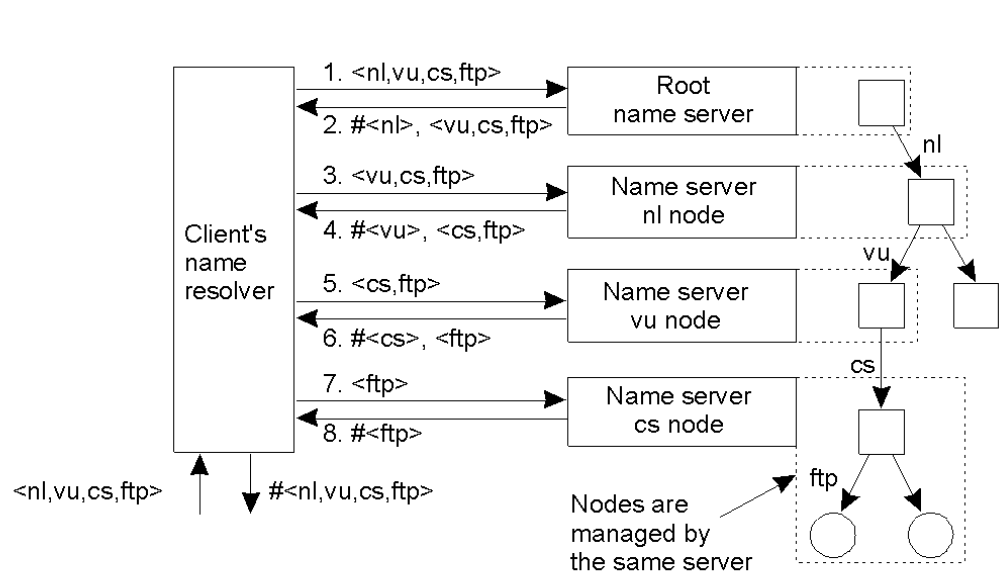
\includegraphics[scale=0.45]{img/iterativa.png}
\caption{Risoluzione dei nomi iterativa}\label{img:iterativa}
\end{figure}
In alternativa al meccanismo iterativo è possibile usare la ricorsione, invece di restituire ogni risultato intermedio al client un \emph{name server} passa il risultato al name server successivo. Questo meccanismo mostrato in \figurename\,\ref{img:ricorsiva} è chiamato \textbf{risoluzione dei nomi ricorsiva.} In questo caso quando il root name server trova l'indirizzo del server che implementa il nodo chiamato \emph{nl} gli chiede di risolvere il path $nl:<vu,cs,ftp,pub,globe,index.html>$, il quale a sua volta individuerà il server che implementa \emph{vu} e gli chiederà di risolvere il rimanente path.\\
L'inconveniente di questo tipo di risoluzione è che richiede ai name server livelli prestazionali maggiori rispetto alla versione iterativa.
\begin{figure}[htb]
\centering
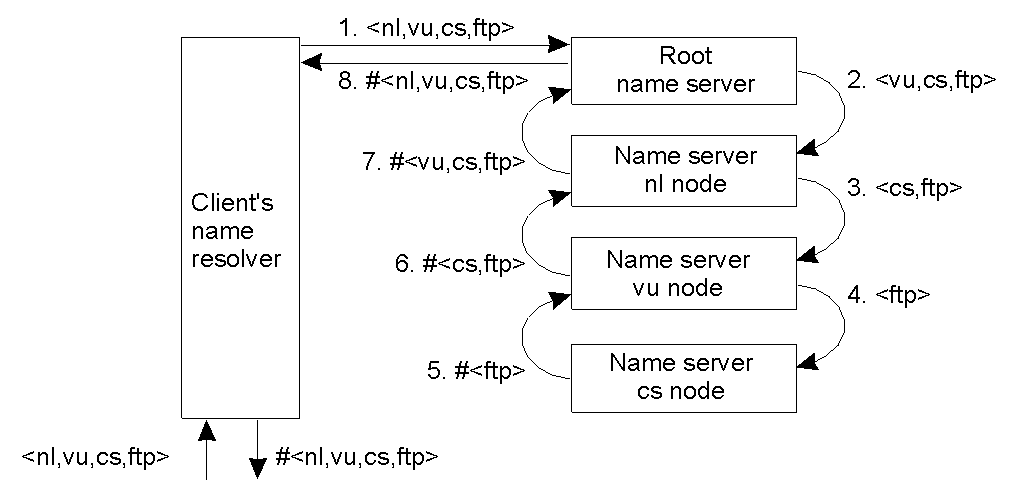
\includegraphics[scale=0.45]{img/ricorsiva.png}
\caption{Risoluzione dei nomi ricorsiva}\label{img:ricorsiva}
\end{figure}
Tuttavia l'approccio ricorsivo presenta anche alcuni vantaggi, ad esempio, il cacheing è molto più efficace rispetto al caso iterativo inoltre, i costi di comunicazione sono ridotti al minimo.
\subsubsection{DNS}
Uno dei servizi di \emph{naming} più diffusi oggi al mondo è il \emph{domain name system} (DNS) di Internet. Il DNS è principalmente usato per ricercare gli indirizzi IP degli host e dei mail server. 
\paragraph{Spazio dei nomi del DNS}
Lo spazio dei nomi del DNS è organizzato gerarchicamente come un albero con radice.
Un'etichetta è una stringa \emph{case insensitive} costituita da caratteri alfanumerici con una lunghezza massima di 63 caratteri; la lunghezza di un path è limitata a 255 caratteri. La rappresentazione di un path name in forma di stringa parte dall'etichetta più a destra e separata da un punto ("."). Anche la radice è rappresentata da un punto ma questo di solito viene omesso. Un esempio è il path name $root:<nl,vu,cs,flits>$ che rappresentato sotto forma di stringa diventa \emph{flits.cs.vu.nl}.\\
Dato che un nodo nello spazio dei nodi ha esattamente un arco in entrata la sua etichetta viene usata come nome del nodo. Un sottoalbero è chiamato \textbf{dominio} ed il path name verso il suo nodo radice è chiamato \textbf{nome del dominio.} Il contenuto di un nodo è costituito da un insieme di \textbf{resource record} i quali possono essere di diverso tipo e sono illustrati in \tablename\,\ref{tab:resource}.
\begin{table}
\centering
\begin{tabular}{|l|l|p{0.5\textwidth}|}
\hline
\textbf{Tipo di record} & \textbf{Entità associata} & \textbf{Descrizone} \\
\hline
SOA & Zona & Informazioni sulla zona rappresentata \\
A & Host & Contiene un indirizzo IP dell'host che questo nodo rappresenta \\
MX & Dominio & Si riferisce ad un mail server che gestisce le mail indirizzate a questo nodo \\
SRV & Dominio & Si riferisce ad un server che gestisce un particolare servizio \\
NS & Zona & Indica il name server che implementa la zona rappresentata \\
CNAME & Nodo & Link simbolico con il nome primario del nodo rappresentato \\
PTR & Host & Contiene il nome canonico dell'host \\
HINFO & Host & Mantiene informazioni sull'host che questo nodo rappresenta \\
TXT & Qualunque tipo & Contiene qualunque tipo di informazione \\
\hline
\end{tabular}
\caption{Tipi importanti di resource record}\label{tab:resource}
\end{table}
Analiziamo ora alcuni campi dei resource record; un campo SOA contiene informazioni quali l'indirizzo mail dell'amministratore di sistema, il nome dell'host dal quale prelevare informazioni sulla zona ecc.
Il resource A(\emph{address}) rappresenta un particolare host in internet, il campo A contiene il suo indirizzo IP, in caso di host \emph{multihomed} un nodo conterrà più campi A.
I record MX (\emph{mail exchange}) sono contengono un link simbolico a un nodo che rappresenta il mail server per quella zona.\\
Un esempio di tali record sono rappresentati in \figurename\,\ref{img:resourcer}
\begin{figure}[htb]
\centering
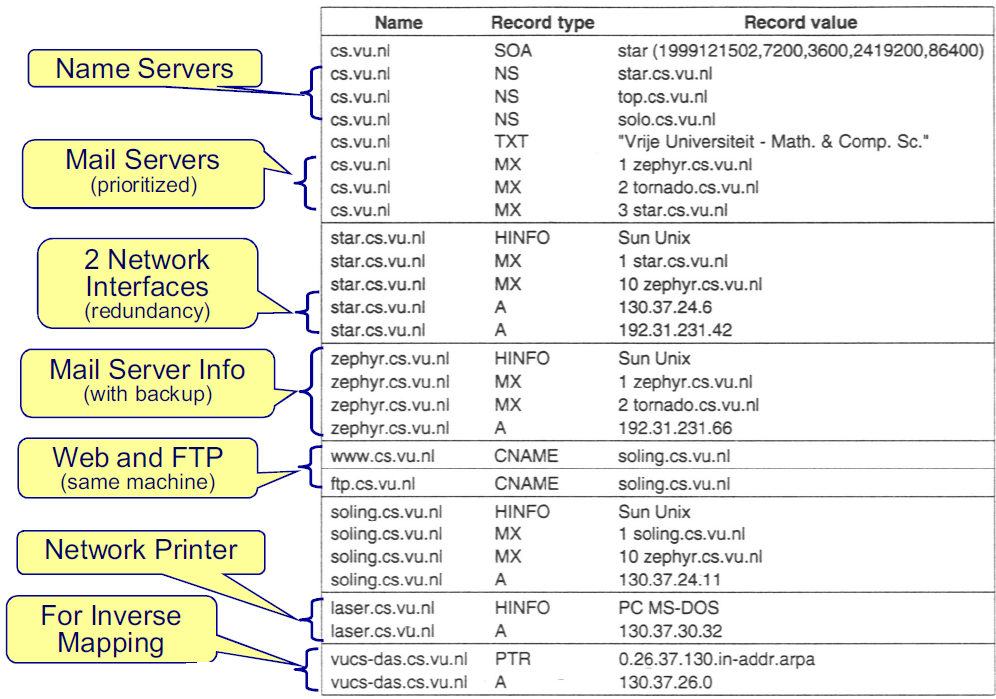
\includegraphics[scale=0.5]{img/resourcer.png}
\caption{Esempio di resource record estratto dalla base di dati per la zona \emph{cs.vu.nl}}\label{img:resourcer}
\end{figure}
\paragraph{Implementazione del DNS}
In sostanza , lo spazio dei nomi del DNS è suddivisibile in un livello globale ed uno amministrativo come mostrato in \figurename\,\ref{img:dnslevel}. Il livello gestionale solitamente è gestito a livello locale e quindi non fa parte del DNS. Ogni zona è implementata da un name server replicato per garantirne la disponibilità. Gli aggiornamenti della zona sono solitamente gestiti dal server primario. Gli aggiornamenti vengono propagati ai server secondari solo tramite richiesta di quest'ultimi, questo procedimento è chiamato \textbf{trasferimento di zona}.\\
Una base di dati del DNS è un insieme di file contenete diversi \emph{resource record} tra questi file uno in particolare contiene gli identificatori di tutti i nodi di una particolare zona in modo da consentire l'identificazione di tutti i nodi semplicemente mediante il nome del loro dominio.
\subsection{Naming basato sugli attributi}
I nomi semplici e quelli strutturati offrono la possibilità di far riferimento ad un'entità in modo indipendente dalla sua posizione. Inoltre i nomi strutturati sono progettati per essere relativamente \emph{human-friendly}. Ma a volte non interessa il nome dell'entità ma un utente vorrebbe ricercare una risorsa in base ad una serie di attributi specificati.\\
Un modo assai diffuso per effettuare questa ricerca è usare un sistema di \textbf{naming basato sugli attributi}, il quale consiste nel descrivere un'entità in termini di coppie (\emph{attributo, valore}) e ad ogni entità possono essere associati più attributi diversi.
\subsubsection{Directory service}
I sistemi di naming basati sugli attributi sono anche conosciuti come \textbf{directory service}. Con questo meccanismo le entità hanno associato un insieme di attributi utilizzabili per le ricerche. Ad esempio in un sistema di mail i messaggi possono essere etichettati tramite attributi relativi al mittente al destinatario all'oggetto e così via; quando però si vuole ampliare il meccanismo dei descrittori risulta un po più difficile, in quanto la maggior parte delle volte tale meccanismo viene impostato manualmente.\\
Per attenuare alcune problematiche sono state introdotti diversi framework tra cui il \textbf{resource description framework} (\textbf{RDF}) il quale basa la sua descrizione su una tripletta formata da soggetto, predicato e oggetto i quali possono essere delle risorse oltre che degli attributi come nel caso della tripletta (\emph{Persona, nome, Alice}) dove si fa riferimento ad una risorsa di tipo \emph{Persona} il cui \emph{nome} è \emph{Alice}.\\
A differenza dei sistemi di naming strutturati la ricerca dei valori in un sistema di naming basato sugli attributi richiede di effettuare una ricerca esaustiva su tutti i descrittori.
\subsubsection{LDAP}
Un approccio diffuso di affrontare il problema dei directory service è quello di combinare il naming strutturato con quello basato sugli attributi, questo approccio è stato ampiamente usato nel servizio \emph{Active Directory} di Microsoft ed in altri sistemi. Molti di questi sistemi utilizzano o si basano sul \textbf{light directory access protocol} comunemente chiamato anche \textbf{LDAP}.\\
Un directory service LDAP consiste in un certo numero di record di solito chiamati elementi della directory. Un elemento della directory è paragonabile ad un resource record del DNS. Ogni record è composto da una coppia (\emph{attributo, valore}) in cui ogni attributo ha un tipo associato. L'insieme di tutti gli elementi di un directory service LDAP è chamato \textbf{directory information base} (\textbf{DIB}). Un aspetto importante di un DIB è che ogni record ha un nome univoco in modo da renderlo identificabile, tale nome appare in ogni record come la sequenza di attributi di naming. Ogni attributo di naming è chiamato \textbf{relative distinguished name} o in breve \textbf{RDN}. Come nel caso dei nomi univoci strutturati l'uso dei nomi globali ottenuti tramite l'elenco degli RDN in sequenza genera una gerarchia degli elemnti della directory chiamata anche \textbf{directory information tree} (\textbf{DIT}). Un DIT non è altro che un grafo dei nomi in un sistema basato su LDAP in cui ogni nodo è un elemento della directory. In tal senso alcuni nodi possono agire sia da elemento sia da directory nel senso tradizionale del termine. Per accedere a tali elementi possiamo utilizzare due distinte  funzioni di interrogazione, la \texttt{read} che è utilizzata per leggere il contenuto di un elemento, e la \texttt{list} utilizzata per elencare i diversi archi in uscita come mostrato in \figurename\,\ref{fig:readlist}.
\begin{figure}[hbt]
\subfigure[]{
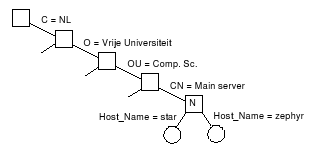
\includegraphics[width=7.5cm]{img/dit.png}
\label{fig:dit}
}
\subfigure[]{
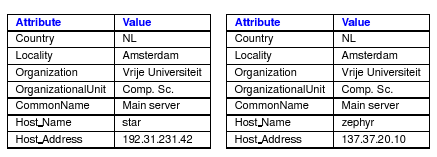
\includegraphics[width=7.5cm]{img/readlist.png}
\label{fig:readlist}
}
\caption{Esempio di DIT \ref{fig:dit} e di valori restituiti da un operazione di list e di read \ref{fig:readlist}}
\end{figure}
Quando si ha progetta un sistema basato su LDAP di larga scala il DIT viene suddiviso su più server chiamati \textbf{directory server agent (DSA)} mentre i client sono chiamati \textbf{directory user agent} o DUA i quali sono simili ai name resolver nel sistema DNS.
\subsection{Removing}
I sistemi di naming fin qui descritti permettono l'accesso a delle entità distribuite molte volte in maniera globale. Ma quando queste entità non vengono più referenziate devono essere eliminate, per fare ciò solitamente si utilizza un garbage collector ma in un ambiente distribuito le cose si complicano alquanto.\\
Esistono tuttavia diversi meccanismi per capire se un entità è ancora differenziata.
\subsubsection{Reference counting}
In questo meccanismo gli oggetti tengono conto di quanti altri oggetti possiedono un loro riferimento, il sistema risulta molto efficiente se il conteggio è fatto tramite l'invio di un solo messaggio come mostrato in \figurename\,\ref{fig:referencecounting} (a) ma purtroppo si potrebbero verificare dei problemi di \emph{race condition} quando si passano dei riferimenti tra processi. Una tecnica è quella di comunicare all'oggetto anche il passaggio di riferimento ad altri processi come mostrato in \figurename\,\ref{fig:referencecounting} (b) questo meccanismoo purtroppo degrada le prestazioni in quanto i messaggi scambianti diventano tre.\\
\begin{figure}[htb]
\centering
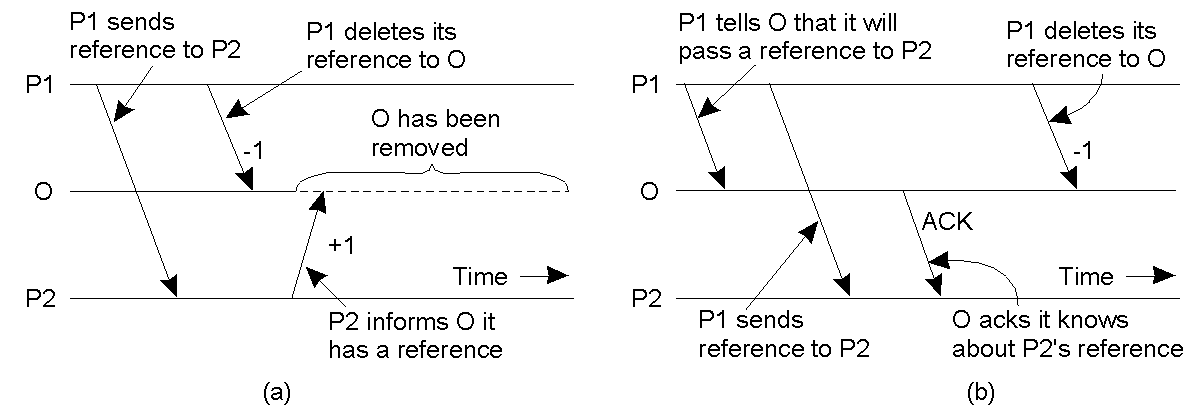
\includegraphics[scale=0.4]{img/referencecounting.png}
\caption{Esempio di reference counting con lo scambio di uno (a) e tre (b) messaggi}\label{fig:referencecounting}
\end{figure}
Un meccanismo simile ma che evita la race condition è quello che utilizza dei pesi per gli oggetti e comunica soltanto il decremento di tali pesi come mostrato in \figurename\,\ref{fig:weight} dove il peso di un oggetto viene diviso tra i due processi che usano tale oggetto, in questo caso al processo $P_2$ il riferimento viene passato dal processo $P_1$. Quando il peso totale e il peso dell'oggetto tornano a pareggiarsi l'oggeto può essere rimosso in quanto non più referenziato. 
\begin{figure}[htb]
\centering
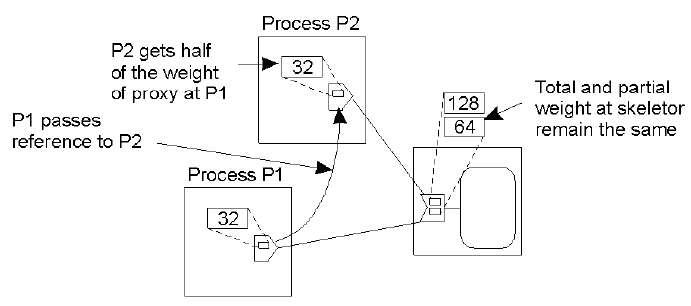
\includegraphics[scale=0.6]{img/weight.png}
\caption{Esempio di reference counting con il meccanismo dei pesi}\label{fig:weight}
\end{figure}
Il problema di questa tecnica è che sono possibili solo un numero limitato di riferimenti. La soluzione è quella di concatenare i riferimenti come mostrato in \figurename\,\ref{fig:weightconcat}; questo risolve il problema dei riferimenti limitati ma aggiunge un hop per l'accesso all'oggetto.
\begin{figure}[htb]
\centering
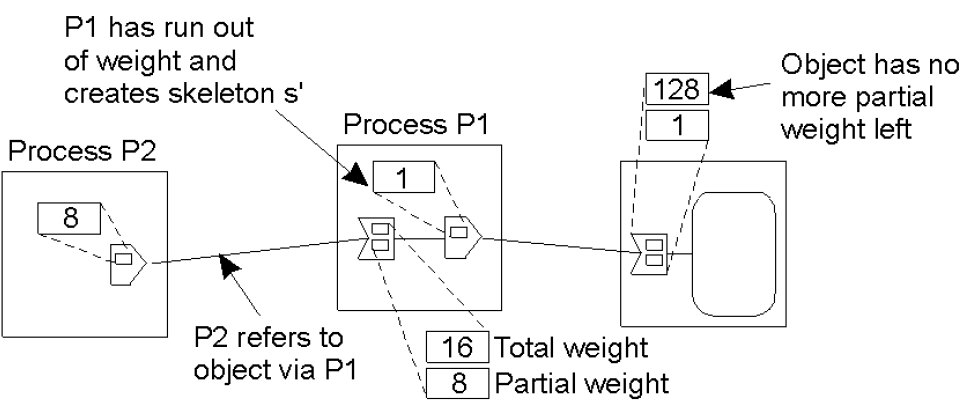
\includegraphics[scale=0.4]{img/weightconcat.png}
\caption{Esempio di reference counting con il meccanismo dei pesi e la concatenazione}\label{fig:weightconcat}
\end{figure}
\subsubsection{Reference listing}
Un altro meccanismo molto utilizzato è quello del reference listing che non tiene traccia del numero di referenze ma soltanto dell'identità di chi richiede un riferimento, il vantaggio è che l'inserimento o l'eliminazione di un proxy (inteso come processo che richiede il riferimento) è idempotente ovvero inserimento e cancellazione di un proxy richiedono un messaggio di ack ma le richieste multiple non hanno effetto sul carico di rete. Il secondo vantaggio è che le risorse orfane possono essere individuate facilmente pingando periodicamente i client presenti nella lista dei riferimenti. Tuttavia anche questo meccanismo soffre del fenomento di race condition quando viene copiato un riferimento.
\subsubsection{Distributed mark-and-sweep}
Il mark and sweep permette di tenere traccia di quelle entità orfane. Nel caso di sistema uniprocessore tale meccanismo si suddivide in due fasi, nella prima fase vengono marchiate tutte le entità accessibili da qualche tipo di referenza. Tutti i nodi partono colorati di bianco, un nodo viene colorato di grigio quando è possibile raggiungerlo dalla root ma alcune delle sue referenze non sono ancora state valutate, infine viene marcato di nero se tutte le sue referenze sono marchiate di grigio.\\
Nella seconda fase il garbage collector elimina tutti i nodi marchiati di bianco.\\
Nel caso di sistema distribuito il garbage collector entra in funzione su ogni nodo, partendo da un nodo P una risorsa viene marchiata di grigio se è possibile raggiungerla dalla root del nodo P quando un proxy $q$ è marchiato di grigio si invia un messaggio a tutti i suoi riferimenti. Quando tutti i riferimenti rispondono con un ack il proxy $q$ viene marchiato di nero.